\documentclass{beamer}
\usepackage{beamerthemeshadow}
\beamersetuncovermixins{\opaqueness<1>{25}}{\opaqueness<2->{15}}
\beamertemplatenavigationsymbolsempty  % Hide beamer control

\setbeamertemplate{footline}[title, frame number]

% Encoding
\usepackage[utf8]{inputenc} % für input utf8
\usepackage[T1]{fontenc}    % Schriftcodierung mit UTF-8
\usepackage{textcomp}       % Erweiterung von fontenc
\usepackage{lmodern}        % Erweiterung des Zeichensatzes



% Anpassungen für die Deutsche
\usepackage[ngerman]{babel} % Neue deutsche Rechtschreibung

\usepackage{ulem}           % Strike trough text

\usepackage{listings}       % Codesegments   
\lstset{language=C}         % Set everything as C code
%\lstset{aboveskip=-11pt}   % Removes Title page for code Blocks

\usepackage{bera}           % Monospace

\begin{document}


% ******** TITLE ********
\title{Quadcopter}  
\author{Pascal Häfliger, Cyrill Knüsel}
\date{\today} 

\begin{frame}
\titlepage
\end{frame} 
\section{Dji 450}

\begin{frame}
\tableofcontents[
    currentsection, 
    %hideothersections, 
    sectionstyle=show/shaded, 
    subsectionstyle=hide
]
\end{frame}







% ******** INTRO ********
\section{Dji 450}

\begin{frame}
\tableofcontents[
    currentsection, 
    %hideothersections, 
    sectionstyle=show/shaded, 
    subsectionstyle=hide
]
\end{frame}






	

% ******** HOW IT WORKS ********
\section{Dji 450}

\begin{frame}
\tableofcontents[
    currentsection, 
    %hideothersections, 
    sectionstyle=show/shaded, 
    subsectionstyle=hide
]
\end{frame}







% ******** OUR COPTER ********
\section{Dji 450}

\begin{frame}
\tableofcontents[
    currentsection, 
    %hideothersections, 
    sectionstyle=show/shaded, 
    subsectionstyle=hide
]
\end{frame}





\subsection{Can}


\begin{frame}
  Compromise between:
  \begin{itemize}
    \item Flight time
    \item Agility
    \item Durability
    \item Control
	\item (Money)
		
  \end{itemize}
\end{frame}



\begin{frame}
\frametitle{Self build kit}

  \begin{itemize}
    \item No special knowledge required    
	\item Very sturdy
	\item A lot of auxiliary
	\item Payload    
	\item Price-Performance ratio
  \end{itemize}
  
\end{frame}



\begin{frame}
\frametitle{Payload}

  \begin{figure}
  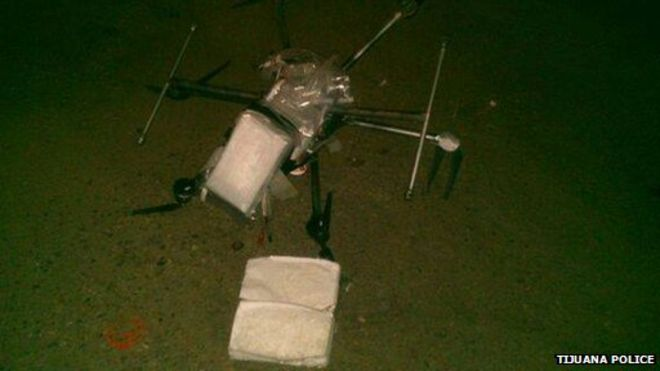
\includegraphics[scale=0.65]{pic/03_our-copter/drug.jpg}
  \end{figure}
  
\end{frame}



\begin{frame}
\frametitle{Controller, modes}

  \begin{itemize}
    \item Manual    
    \item Stabilize    
	\item Follow + obstacle avoidance
	\item Acrobat 	
    \item Way-points   
	\item 6 additional modes 
  \end{itemize}
  
\end{frame}



\begin{frame}
\frametitle{Tools, way-point}

  Configure and calibration
  \begin{figure}
  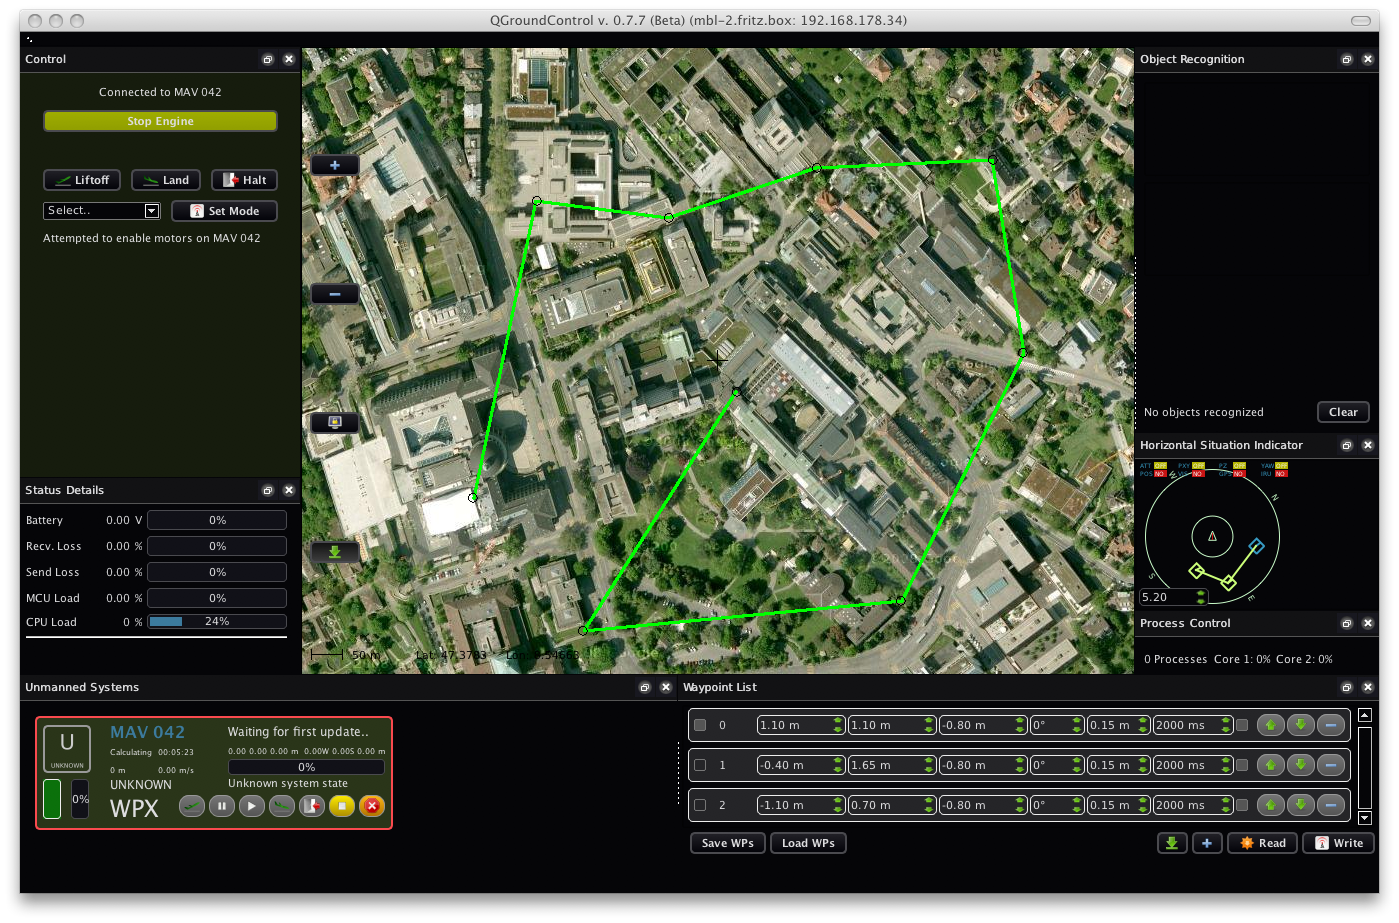
\includegraphics[scale=0.19]{pic/03_our-copter/qgroundcontrol.png}
  \end{figure}
  
\end{frame}



\begin{frame}
\frametitle{Gimbal}

  \begin{figure}
  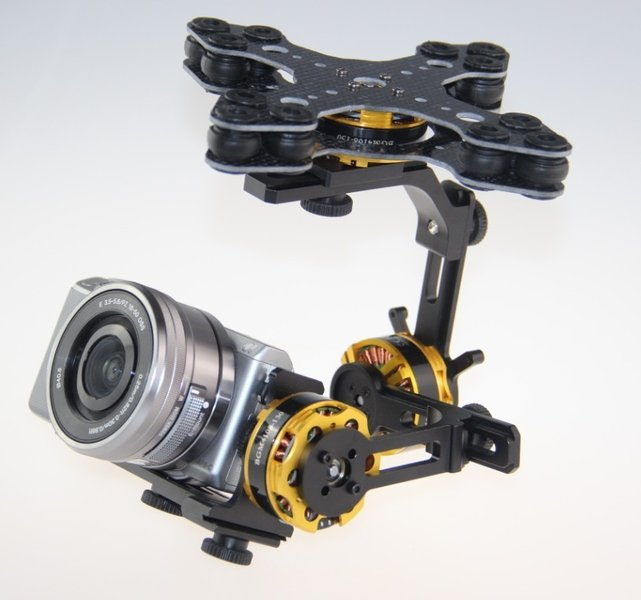
\includegraphics[scale=0.5]{pic/03_our-copter/gimbal.jpg}
  \end{figure}
  
\end{frame}



\begin{frame}
\frametitle{FPV - First Person View}

  \begin{itemize}
    \item Goggle with receiver
  	\item Camera with transmitter
	\item Black \& white picture
	\item Noise 
  \end{itemize}
  
\end{frame}


%\begin{frame}
%\frametitle{FPV - First Person View}

  %	Add picture from FPV
  %\begin{figure}
  %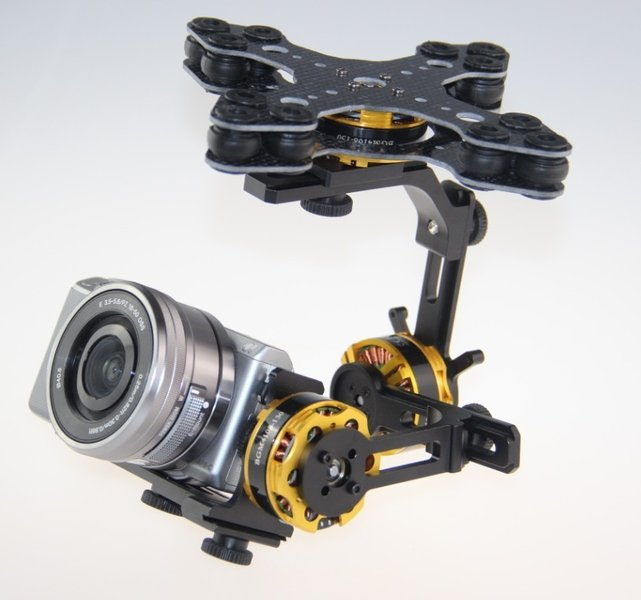
\includegraphics[scale=0.4]{pic/03_our-copter/gimbal.jpg}
  %\end{figure}
  
%\end{frame}


\subsection{Can not}

\begin{frame}
\frametitle{....}

  %\begin{figure}
  %\includegraphics[scale=0.6, trim={5cm 8.5cm 5.5cm 8.5cm},clip]{pic/03_content/Serial_output.pdf}
  %\end{figure}
  
\end{frame}


\begin{frame}
\frametitle{Controller}

  \begin{itemize}
    \item ...
  \end{itemize}
    
\end{frame}
\subsection{Limitations}

\begin{frame}
\frametitle{Power supply}

  \begin{itemize}
    \item Li-Po Battery: ~14V, 5Ah $\rightarrow$ 0.055 kWh
    \item Flight time: 5min - 20min
    \item Charge time: about 2 hours
	\item Gasoline
  \end{itemize}
  
\end{frame}



\begin{frame}
\frametitle{Power supply}

  \begin{figure}
  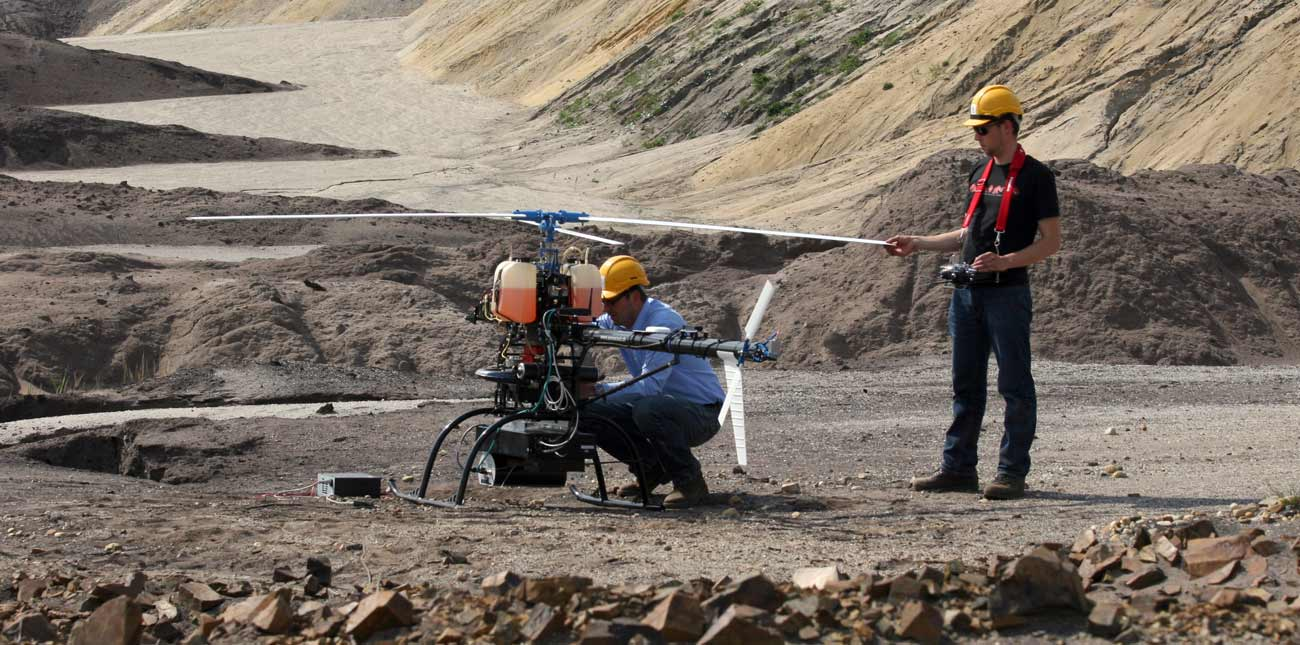
\includegraphics[scale=0.24]{pic/03_our-copter/aeroscout.jpg}
  \end{figure}
  
\end{frame}



\begin{frame}
\frametitle{Distance}

  \begin{itemize}
    \item 1.2 miles normal
    \item 6.2 miles Yagi antenna
  \end{itemize}
  
  % Yagi antenna picture
    
\end{frame}



\begin{frame}
\frametitle{Law, Risk towards others}

  \begin{itemize}
    \item Register devices    
	\item Fish drones from sky
  \end{itemize}
  	
	% eagle.jpeg
	% net.jpg
	% turtle.png
	% latest news from heathrow was a plastic bag --> register all pastic bags
	%
\end{frame}



\begin{frame}
\frametitle{Law, Risk towards others}
  
  \begin{figure}
  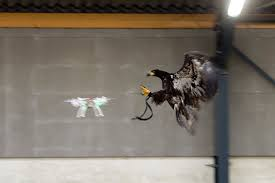
\includegraphics[scale=0.9]{pic/03_our-copter/eagle.jpeg}
  \end{figure}

\end{frame}



\begin{frame}
\frametitle{Law, Risk towards others}
  
  \begin{figure}
  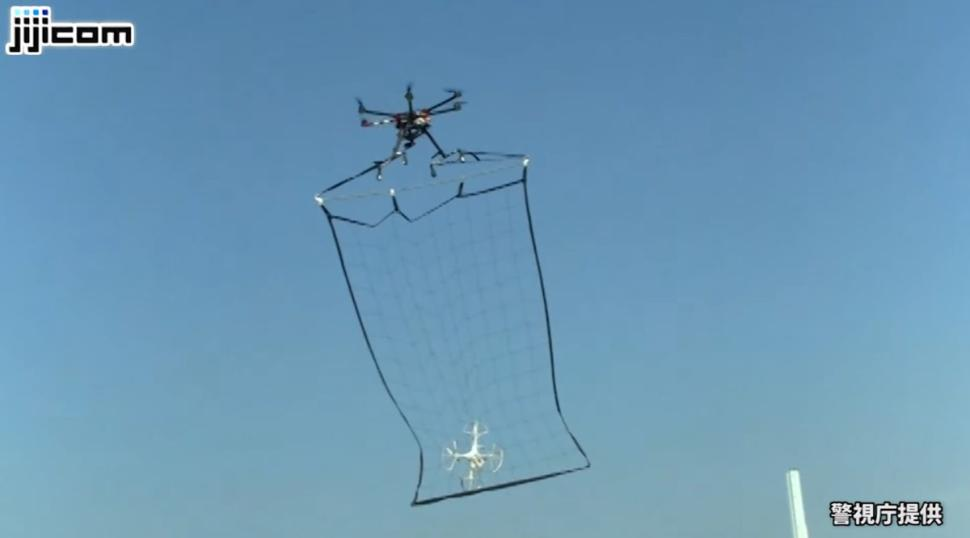
\includegraphics[scale=0.31]{pic/03_our-copter/net.jpg}
  \end{figure}

\end{frame}



\begin{frame}
\frametitle{Law, Risk towards others}
  
  \begin{figure}
  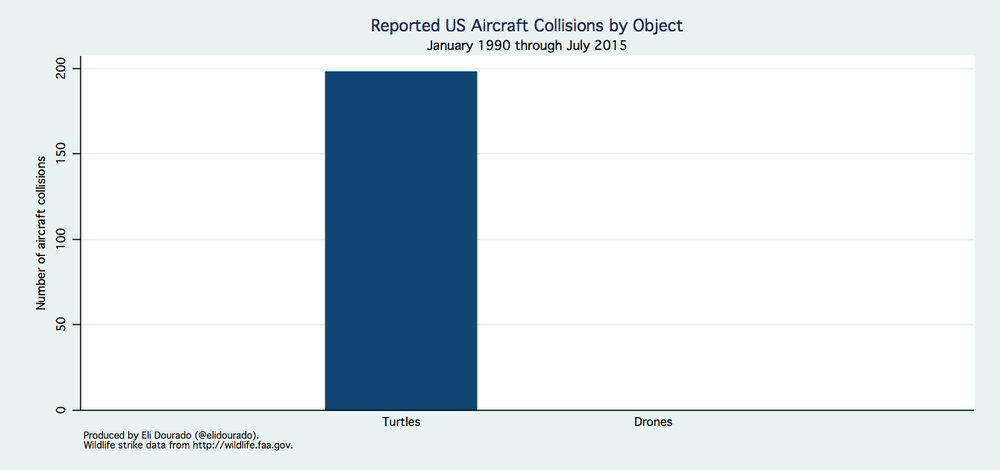
\includegraphics[scale=0.3]{pic/03_our-copter/turtle.png}
  \end{figure}

\end{frame}



% ******** USAGE ********
\section{Dji 450}

\begin{frame}
\tableofcontents[
    currentsection, 
    %hideothersections, 
    sectionstyle=show/shaded, 
    subsectionstyle=hide
]
\end{frame}





\subsection{Personal Usage}

\begin{frame}
\frametitle{....}

  \begin{itemize}
    \item ....    
  \end{itemize}
  
\end{frame}





%\subsection{Professional Usage}



%\begin{frame}
%\frametitle{Testing}
%
%  \begin{itemize}
%  	\item Cheap version of a quad 
%    \item Test new control software
%    \item Allowed to crash  
%  \end{itemize}
%  
%\end{frame}



%\begin{frame}
%\frametitle{Education}
%
%  \begin{itemize}
%  	\item Software and Hardware is changeable, expandable
%  	\item A good mix of everything
%  	\item Mostly indoors
%  \end{itemize}
%  
%\end{frame}



% ******** CONCULSION ********
\section{Dji 450}

\begin{frame}
\tableofcontents[
    currentsection, 
    %hideothersections, 
    sectionstyle=show/shaded, 
    subsectionstyle=hide
]
\end{frame}






	


\end{document}